\documentclass[conference]{IEEEtran}

\usepackage{amsmath,amssymb,amsfonts}
\usepackage{algorithmic}
\usepackage{subcaption}
\usepackage{graphicx}
\usepackage{hyperref}
\usepackage{textcomp}
\usepackage{xcolor}
\usepackage{svg}
\usepackage[style=ieee]{biblatex}

\addbibresource{references.bib}

\def\ns3{ns-3}

\begin{document}

\title{Extending Energy Models for Wireless Network Simulation with FMI-based Hybrid Co-Simulation}

\author{\IEEEauthorblockN{Lars Moons}
\IEEEauthorblockA{\textit{Department of Computer Science} \\
\textit{University of Antwerp}\\
lars.moons@student.uantwerpen.be}
}

\maketitle

\begin{abstract}
This paper proposes a novel workflow for extending energy models in wireless network simulation using hybrid co-simulation based on the Functional Mock-up Interface (FMI). Currently, adding new energy models to the \ns3 energy framework requires a tedious workflow involving creating a circuit diagram, solving the circuit and writing the code, which can be time-consuming and error-prone. To address these challenges, the proposed workflow integrates visual design, drag-and-drop functionality, and predefined model building blocks from tools like OpenModelica and Simscape, which will interact with discrete-event simulators like \ns3 through FMI.
\end{abstract}

\begin{IEEEkeywords}
energy modelling, \ns3, hybrid co-simulation, FMI, wireless network simulation 
\end{IEEEkeywords}

\section{Introduction}

Energy modelling is a critical aspect of evaluating the performance of wireless network protocols.
Therefore, in the network simulator \ns3, a generic energy framework is provided, with basic structures for modelling energy sources \cite{wu2012energy}.
While there are some pre-built models available, more advanced energy models require programmers to write their own code.
In a previous study \cite{capuzzo2021ns}, the authors encountered this situation, when they modelled a battery-less IoT device with energy harvesting using the \ns3 energy model interface.
Their workflow involved creating a circuit diagram, solving the circuit using analysis techniques, and implementing the resulting formula in code. 
This approach proves effective for smaller and less complex circuits.
However, when more realism is necessary, this workflow becomes challenging due to potential errors, time consumption, and unfamiliarity with circuit analysis techniques. Furthermore, integrating energy models developed by different teams using different toolsets can pose difficulties.

To overcome these challenges, we propose a new workflow that incorporates visual design, drag-and-drop functionality, and predefined model building blocks \cite{carreira2020foundations}. Existing tools like OpenModelica and Simscape offer such functionality, but they do not directly integrate with discrete-event simulators like \ns3. Hence, the challenge lies in combining these two environments through hybrid co-simulation.
The integration can be made possible with the Functional Mock-up Interface (FMI) standard, which enables communication between the two environments.
Previous work in \cite{cremona2019hybrid}, \cite{cremona2016step}, and \cite{widl2015fmi} has explored FMI-based hybrid co-simulation. \cite{cremona2019hybrid} and \cite{cremona2016step} primarily discuss general implementation details, while \cite{widl2015fmi} delved into a specific use case.
This paper discusses another unexplored use case, namely the application to simulating energy models in wireless network simulations, which makes it a novel contribution in this domain.

In the following sections, we will briefly review discrete-event and physical simulation, discuss the FMI standard, and present the architectural design.
Then, we will demonstrate two proof-of-concept implementations: one based on Python and another based on C++.
Finally, we will talk about future work and conclude the paper.

\section{Background}
\label{section:background}

\subsection{Discrete-Event Simulation}

In a discrete-event, simulation events occur at specific points in time.
Each event marks a change of state in the system, and states can only change when events take place. 
The simulator maintains a queue of events that are scheduled to execute at a specified simulation time.
These events are executed in sequential time order.
After an event is completed, the simulator proceeds to the next event in the queue or terminates if there are no more events remaining.
Discrete-event simulators are often used in network simulators to model events such as
packet transmission or changes in network topology \cite{riley2010ns}.
Two popular open-source frameworks in this domain are \ns3 and OMNeT++.

\begin{figure}[htbp]
  \centering
  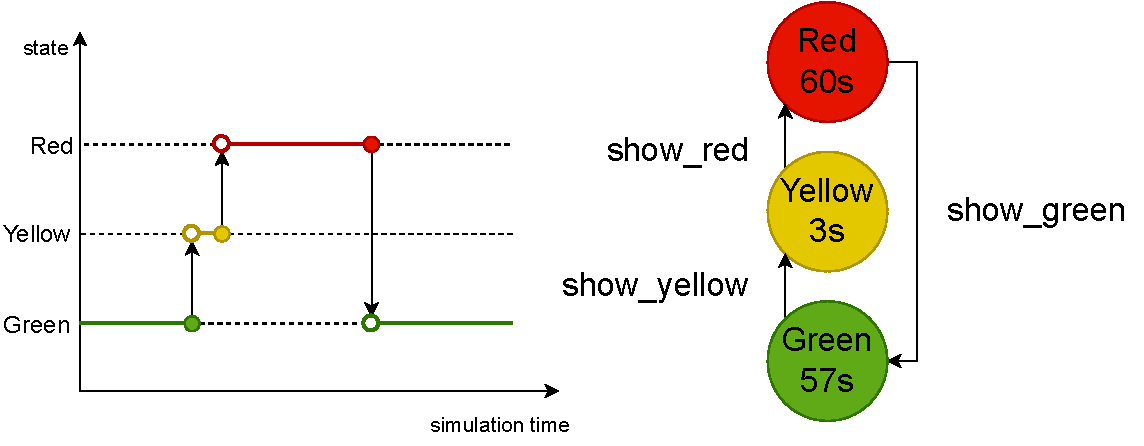
\includegraphics[width=\linewidth]{images/traffic-light.drawio.pdf}
  \caption{Discrete-event system of a traffic light.}
  \label{traffic-light}
\end{figure}

A simple example of a discrete-event system is a traffic light, see Fig. \ref{traffic-light}.
The traffic light has three states: \texttt{RED}, \texttt{YELLOW} and \texttt{GREEN},
and is controlled by three events: \texttt{show\_red}, \texttt{show\_yellow} and \texttt{show\_green}, which set the traffic light to the colour indicated by their names.
The system starts in the \texttt{GREEN} state and schedules the \texttt{show\_yellow} event to occur after 57 seconds.
The simulator advances the simulation time to 57 seconds and executes the \texttt{show\_yellow} event.
During this event, the traffic light transitions to the \texttt{YELLOW} state, and the \texttt{show\_red} event is scheduled to execute after 3 seconds, relative to the current simulation time.
Continuing the simulation, the time is advanced to 60 seconds and the \texttt{show\_red} event is executed.
As a result, the traffic light transitions to the \texttt{RED} state, and the \texttt{show\_green} event is scheduled to execute after 60 seconds.
After that, the simulation time is advanced to 120 seconds, and the \texttt{show\_green} event is executed.
This returns us to the initial state, and the process repeats.

\subsection{Physical Simulation}

Physical simulation employs mathematical equations to model the behaviour of physical objects.
Unlike the discrete events, it operates in a continuous state space.
Two popular tools that support physical simulation are OpenModelica and Simscape.
These tools are available as either open-source software or free for academic research.
They eliminate the need to numerically solve systems of equations that govern the laws of physics.
Instead, they provide pre-written blocks that can be connected graphically and let the solver do all the tedious work.
In addition to their graphical interfaces, these tools also support their own modelling language. These languages resemble regular programming languages but operate at a higher level of abstraction.
They are equation-based rather than assignment-based, enabling acausal data flow that does not fix input or output variables.
This flexibility allows inputs and outputs to be derived depending on the situation.

Let's consider a simple physical system, such as a discharging capacitor, see Fig. \ref{capacitor-discharge}.
The system consists of two main components: a capacitor and a resistor.
Using the aforementioned tools, these components can be connected graphically (Fig. \ref{cd:graphical-model}).
The graphical model is then translated into a textual modelling language (Fig. \ref{cd:modeling-language}), in which the behaviour of a discharging capacitor is described with a differential equation:
\[
\frac{dV}{dt} = -\frac{V}{CR}
\]
Finally (Fig. \ref{cd:numerical-solution}), the equation is solved numerically using Euler's method which approximates the derivative by finite differences:
\[
y'(t_0) \approx \frac{y(t_0+h) - y(t_0)}{h}
\]
Note that this example serves to provide intuition rather than demonstrate the exact working of OpenModelica or Simscape.

\begin{figure}[htbp]
  \centering
  \begin{subfigure}[b]{\linewidth}
    \centering
    \includesvg[width=0.4\linewidth]{images/capacitor-discharge-graphical.svg}
    \caption{Graphical model}
    \label{cd:graphical-model}
  \end{subfigure}
  
  \vspace{1em}
  
  \begin{subfigure}[b]{\linewidth}
    \centering
    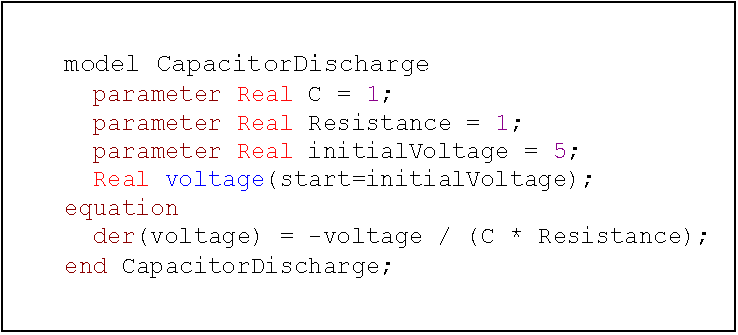
\includegraphics[width=0.9\linewidth]{images/capacitor-discharge-code.drawio.pdf}
    \caption{Modelling language}
    \label{cd:modeling-language}
  \end{subfigure}
  
  \vspace{1em}
  
  \begin{subfigure}[b]{\linewidth}
    \centering
    \includesvg[width=0.9\linewidth]{images/capacitor-discharge-plot.svg}
    \caption{Numerical solution}
    \label{cd:numerical-solution}
  \end{subfigure}
  
  \caption{Physical system of a discharging capacitor.}
  \label{capacitor-discharge}
\end{figure}

\subsection{FMI standard}

The Functional Mock-up Interface (FMI) is the de facto standard for co-simulation and model-exchange.
It will enable the integration between discrete-event and physical simulation from the previous sections.
OpenModelica and Simscape have both incorporated FMI into their software platforms, offering support for importing and exporting models.
The FMI specification, currently at version 3.0, provides a generic and powerful interface
However, as tooling support is still evolving, we will focus on Version 2.0, which includes all the necessary features for our specific use-case.
FMI defines two types of interfaces, FMI for Co-Simulation (CS) and FMI for Model Exchange (ME).
While CS operates as a stand-alone black-box, ME requires an external numerical solver.
For our implementation, we use the CS type as it offers sufficient functionality.

A Functional Mock-up Unit (FMU) encapsulates a model that exposes the FMI interface.
It is packaged as a ZIP file containing an XML-based model description and a shared library that implements the FMI interface as a C API, as in Fig. \ref{FMU-architecture}.
Additionally, an FMU may include source code and documentation.
The shared library could be compiled from a single C source file.
However, in practice, the functionality is often decomposed into three components: the FMI source, which precisely defines the functions according to the FMI standard; the co-simulation source, which includes a numerical solver used by all CS models; and the model source, which contains code specific to the particular physical system being modelled.

\begin{figure}[htbp]
  \centering
  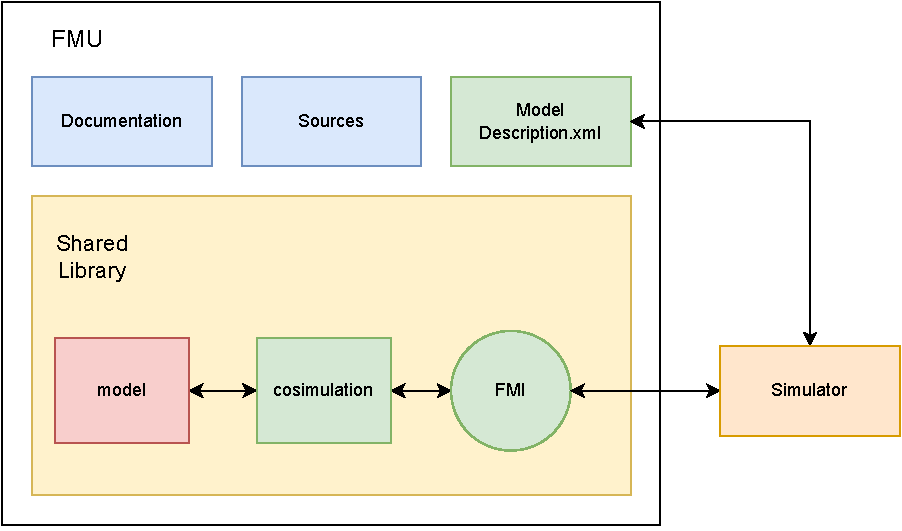
\includegraphics[width=\linewidth]{images/FMU-architecture.drawio.pdf}
  \caption{Components of the FMU architecture.}
  \label{FMU-architecture}
\end{figure}

\section{Architectural Design}

We can combine the three components discussed in the \nameref{section:background} section into a cohesive architecture, as illustrated in Figure \ref{architectural-design}. This architecture combines Discrete-Event Simulation, Physical Simulation, and the FMI standard.

To summarise, discrete-event frameworks such as \ns3 and OMNeT++ run simulators that continuously loop and trigger events. Within these events, models written in these frameworks are called for their specific functionality. These models have energy components, which are controlled through the FMI interface. On the other end of the interface, we find the energy models originally exported from tools like OpenModelica and Simscape, completing the architecture.

\begin{figure}[htbp]
  \centering
  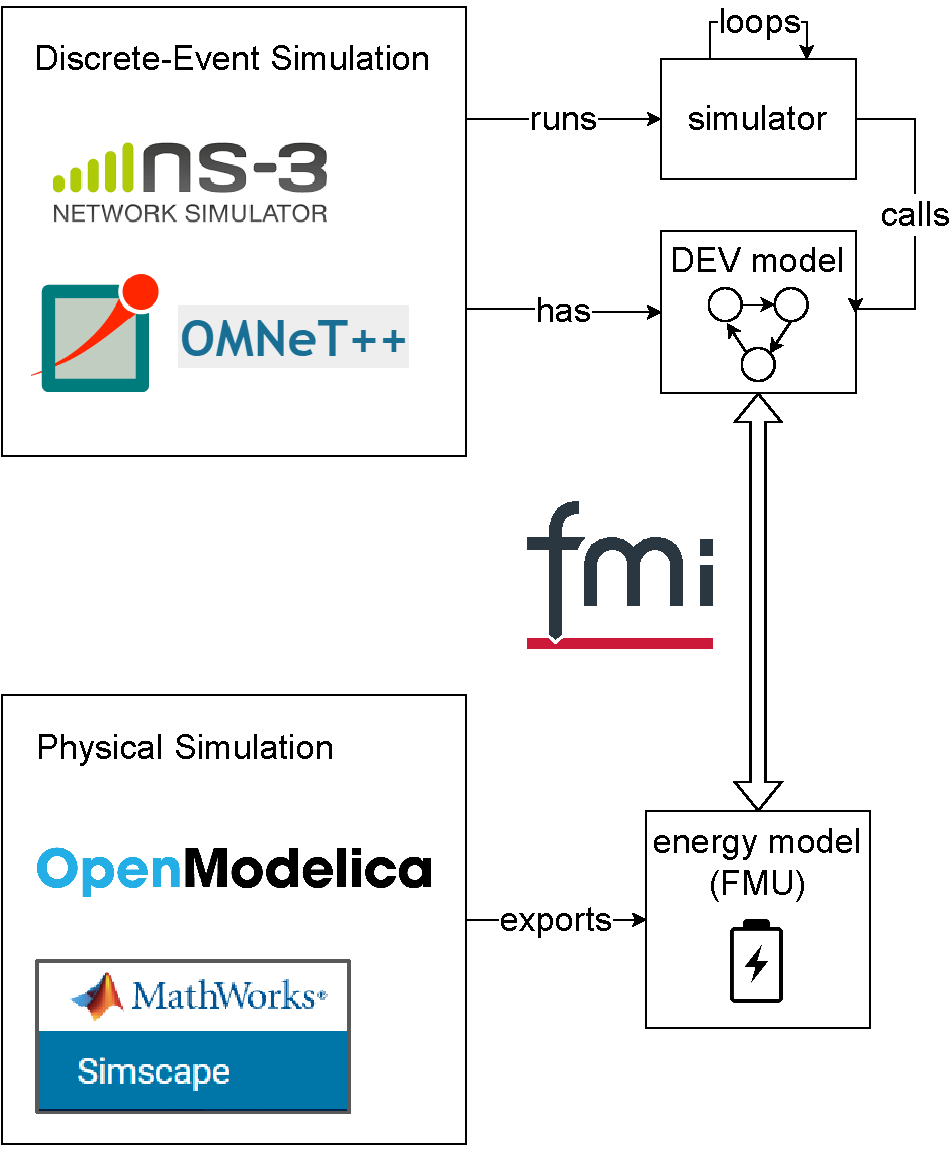
\includegraphics[width=0.8\linewidth]{images/architectural-design.drawio.pdf}
  \caption{Architectural Design Diagram.}
  \label{architectural-design}
\end{figure}

\section{Implementation}

This section presents two proof-of-concept implementations that can be found on Github \footnote{https://github.com/lbm98/devs-fmu}. The first implementation will be in Python, chosen for its simplicity and wide range of available libraries.
Note that this PoC attempts to validate the architecture proposed in the previous section,
and will therefore not include energy components or wireless network nodes.

\subsection{Discrete-Event Simulator PoC}

The discrete-event simulator is implemented as a Python class with the following methods:
\begin{itemize}
    \item \texttt{schedule}: Places an event into the queue based on its scheduled time.
    \item \texttt{run}: Executes the simulation by executing and scheduling new events. It continues until there are no events left or a stop condition is met.
    \item \texttt{advance}: Advances the simulation time by \texttt{t} seconds by running the simulation for \texttt{t} seconds.
    \item \texttt{reset}: Clears the event queue and resets the simulation time to 0 seconds.
\end{itemize}

\subsection{Physical Simulator PoC}

The physical simulator component is straightforward, as no implementation is required. We only need to download an existing FMU from either the Reference-FMUs project or one exported from OpenModelica.

\subsection{Discrete Event Model PoC}

The discrete-event model is conceptually part of the discrete-event system,
but connects with the physical system through the FMI interface.
In Python, directly interfacing with the C-based FMI is not possible,
so we need a Python binding.
To simplify working with FMU models, such as extracting the ZIP file and parsing the XML description, we use FMPy,
as it is recommended on the official FMI standard website
and is actively maintained.
FMPy provides access to the following functions from the FMI interface:
\begin{itemize}
    \item \texttt{fmi2Instantiate}: initialises the FMU model state.
    \item \texttt{fmi2SetupExperiment}: Sets the simulation start and stop time.
    \item \texttt{fmi2EnterInitializationMode}, \texttt{fmi2ExitInitializationMode}: Do nothing, but are considered good practice to call.
    \item \texttt{fmi2GetReal} Retrieves values from the FMU model state.
    \item \texttt{fmi2SetReal} Sets values of the FMU model state.
    \item \texttt{fmi2DoStep} Simulates the FMU model up to the specified time using a numerical solver like Euler's method.
    \item \texttt{fmi2Terminate}, \texttt{fmi2FreeInstance}: Cleans up the model by freeing memory 
    
\end{itemize}
For a sequence diagram, refer to Fig. \ref{fmi-sequence} and
for an overview of the architecture, refer to Fig. \ref{python-implementation-architecture}.

\begin{figure}[htbp]
  \centering
  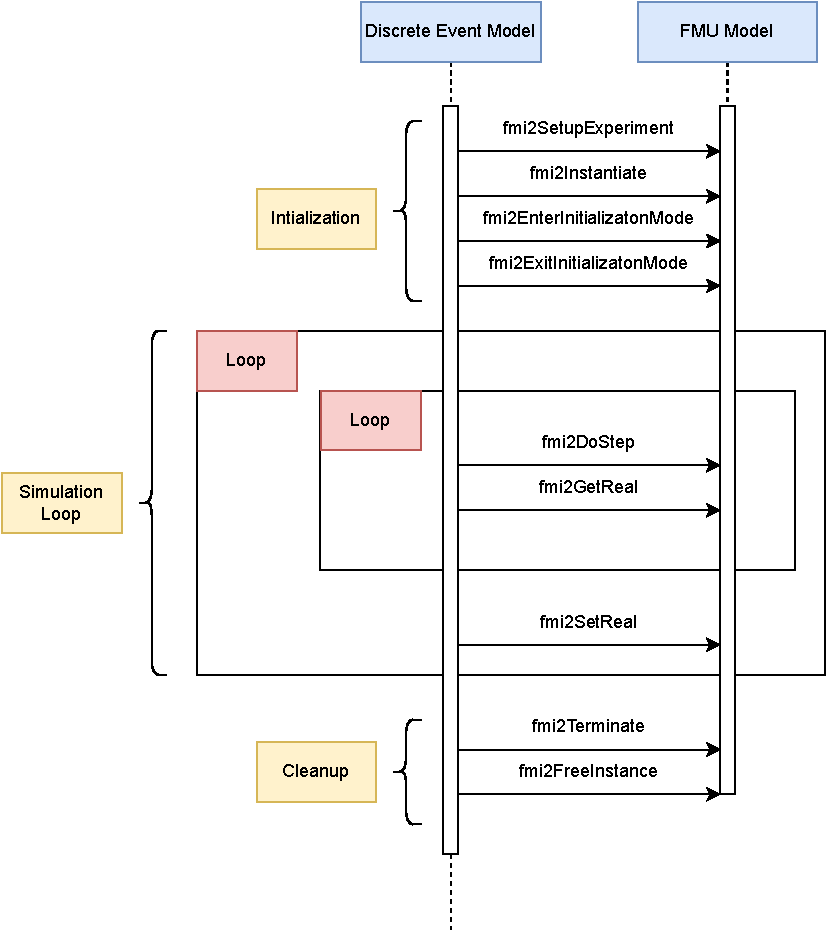
\includegraphics[width=\linewidth]{images/fmi-sequence.drawio.pdf}
  \caption{Sequence diagram of FMI interaction.}
  \label{fmi-sequence}
\end{figure}

\begin{figure}[htbp]
  \centering
  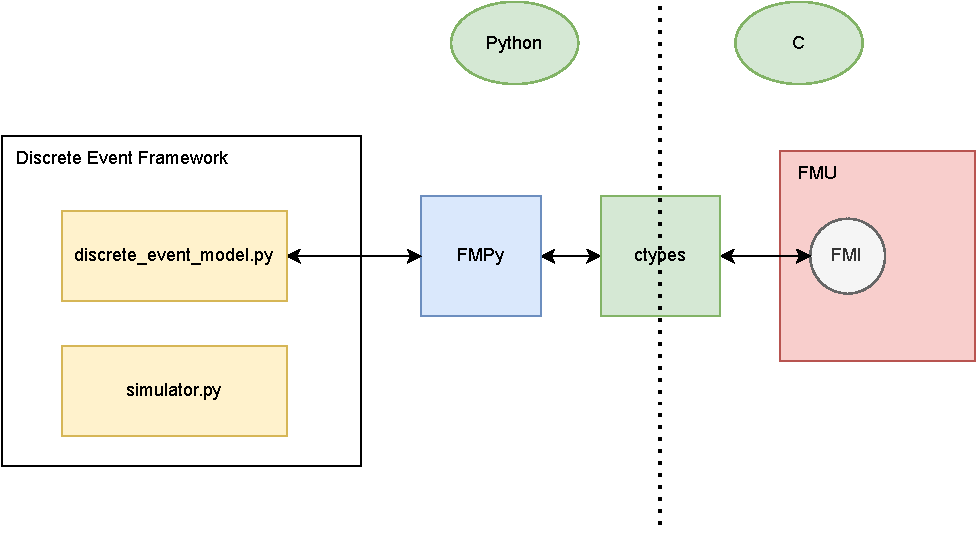
\includegraphics[width=\linewidth]{images/python-implementation-architecture.drawio.pdf}
  \caption{Python implementation architecture.}
  \label{python-implementation-architecture}
\end{figure}

\subsection{Bouncing Ball FMU}

To provide a concrete example, let's consider a model of a bouncing ball.
The model was taken from the Reference-FMUs project, which contains hand-coded FMUs for testing and debugging.
The behaviour of the bouncing ball is described by two differential equations:
\[
\begin{cases}
\frac{dh}{dt} = v \\
\frac{dv}{dt} = g
\end{cases}
\]
relating height, velocity, and acceleration, along with two when-conditions
\[
\begin{aligned}
&\text{when } h \leq 0 \text{ then} \\
&\quad \begin{cases}
h := 0 \\
v := -e \cdot v
\end{cases} \\
&\text{when } v < v_{\text{min}} \text{ then} \\
&\quad \begin{cases}
h := 0 \\
v := 0
\end{cases}
\end{aligned}
\]
where $e$ is the coefficient of restitution.
The Github repository provides notebooks that visualise the behaviour of the bouncing ball by plotting its height over time, also shown in Fig. \ref{fmu-comparsion-no-event}.
During the simulation, no discrete-events occurred, but the next experiment adds an event that resets the height and velocity to their initial values, see Fig. \ref{fmu-comparsion-with-event}.
In both figures, we compare the Reference FMU with an FMU generated by OpenModelica, for the same bouncing ball model, and the resulting behaviour is shown to be similar.

\begin{figure}[htbp]
  \centering
  \begin{subfigure}[b]{\linewidth}
    \centering
    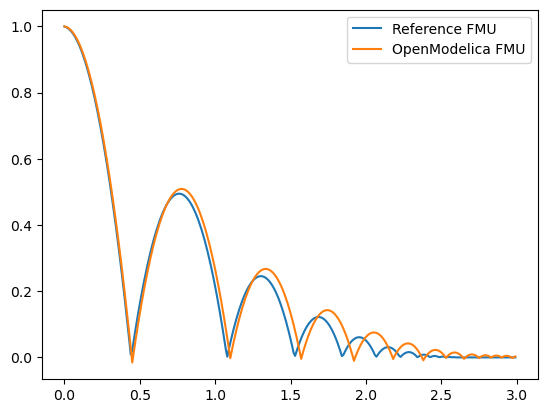
\includegraphics[width=0.5\linewidth]{images/fmu-comparsion-no-event.png}
    \caption{Default simulation}
    \label{fmu-comparsion-no-event}
  \end{subfigure}
  
  \vspace{1em}
  
  \begin{subfigure}[b]{\linewidth}
    \centering
    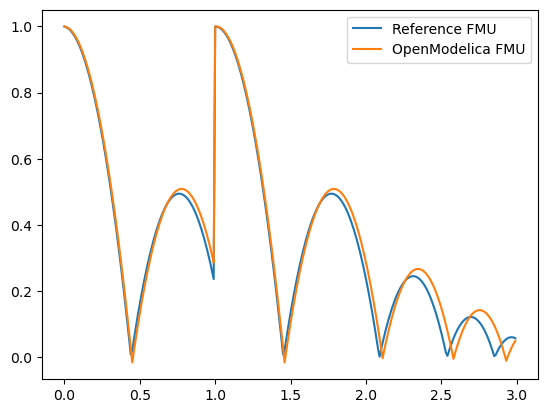
\includegraphics[width=0.5\linewidth]{images/fmu-comparsion-with-event.png}
    \caption{Simulation with reset event}
    \label{fmu-comparsion-with-event}
  \end{subfigure}
  
  \caption{Bouncing ball simulated with Reference FMU and OpenModelica FMU.}
  \label{comparsion-ref-om}
\end{figure}

\subsection{Implementation in C++}

The target discrete-event frameworks \ns3 and OMNeT++ are written in C++.
Integrating  a Python runtime into the simulation would add significant overhead.
Therefore, progress has been made on the C++ implementation, but it is still in the early stages. This brings us to future work.

\section{Future Work}

In future work, we plan to test additional models using both the Python and C++ implementations. This will help us verify their compatibility, performance and possible complications.
Our overarching goal is to create a comprehensive library of energy models saved as OpenModelica or Simscape graphical models, that will seamlessly integrate with \ns3, enriching its energy model framework in a user-friendly, maintainable, and flexible way.

\section{Conclusion}
In conclusion, this paper proposes a workflow that combines discrete-event simulation with physical simulation using the Functional Mock-up Interface (FMI). By integrating visual design and drag-and-drop functionality from tools like OpenModelica and Simscape with discrete-event simulators like ns-3, advanced energy models can be created more effectively. The PoC implementation in Python demonstrates the feasibility of the approach, and work is underway to develop a C++ implementation for integration with ns-3. This workflow has the potential to enhance energy modelling in wireless network simulations and could ultimately lead to a comprehensive library of user-friendly, maintainable, and flexible energy models.

\printbibliography

\end{document}
